\documentclass[12pt, a4paper, oneside]{ctexart}
\usepackage{graphicx}
\usepackage{float}
\usepackage{wrapfig}
\usepackage{color}
\usepackage{xcolor}
\linespread{1.1}
\usepackage{geometry}
\geometry{a4paper,scale=0.8}
\title{历史资料整理}
\author{史成鉴}
\date{}
\begin{document}
	\maketitle
	\newpage
	\tableofcontents
	\newpage
	\section{七年级下 \ 第一单元 \ 隋唐时期：繁荣与开放的时代}
	\begin{enumerate}
		\item 隋唐时期的时代特征：\underline{\textbf{繁荣与开放}}
		\item 对内关系：民族关系（汉族与少数民族）\\ 对外关系：中外关系（中国与外国）
		\item 唐朝实行\underline{\textbf{开明的民族政策}}、\underline{\textbf{开放的对外政策}}
	\end{enumerate}
	
	\subsection{隋朝的统一与灭亡}
	
	\begin{enumerate}
		\item 隋朝的建立和统一
		\begin{enumerate}
			\item 隋朝的建立：\underline{\textbf{581}}年，\underline{\textbf{杨坚}}建立隋朝，定都\underline{\textbf{大兴}}，杨坚就是\underline{\textbf{隋文帝}}
			\item 隋朝的统一：\underline{\textbf{589}}年，\underline{\textbf{隋文帝}}灭掉陈朝，统一全国 \\ 意义：隋的统一，结束了长期分裂的局面，顺应了统一多民族国家的历史发展趋势。
			\item 隋文帝巩固政权的措施
				\begin{enumerate}
					\item 经济上：发展经济，编订户籍，统一南北币制和度量衡制度；
					\item 政治上：加强中央集权，提高行政效率。（确立了\underline{\textbf{三省六部制}}）
				\end{enumerate}
				作用：促进了社会经济的迅速恢复和发展，使\underline{\textbf{人口数量}}和\underline{\textbf{垦田面积}}大幅度增长，隋朝成为疆域辽阔、国力强盛的王朝。隋文帝统治时期的治世局面被称为：\underline{\textbf{开皇之治}}
		\end{enumerate}
		\item 开通大运河（隋炀帝）
			\begin{enumerate}
				\item 目的：为了加强南北交通，巩固隋王朝对全国的统治
				\item 概况：隋炀帝从605年起陆续开凿了长达2700多千米，是古代世界上最长的运河。
					\begin{enumerate}
						\item 三点：以\underline{\textbf{洛阳}}为中心，北达\underline{\textbf{涿郡}}（今北京），南至，\underline{\textbf{余杭}}（今杭州）。
						\item 四段：从北向南依次是\underline{\textbf{永济渠、通济渠、邗沟、江南河}}。
						\item 五河：从北向南依次是\underline{\textbf{海河、黄河、淮河、长江、钱塘江}}五大水系。
					\end{enumerate}
					\begin{figure}[H]
						\centering
						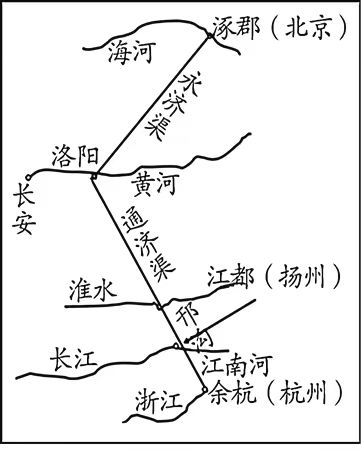
\includegraphics[scale=0.5]{img/101.png}
						\caption{大运河}
					\end{figure} 
				\item 开通的作用
					\begin{enumerate}
						\item 积极作用：加强了南北地区的政治、经济和文化交流。
						\item 消极作用：给百姓带来了沉重负担，加速了隋朝的灭亡。
					\end{enumerate}
			\end{enumerate}
		\item 开创科举取士制度（隋炀帝）
			\begin{enumerate}
				\item 初步建立：\underline{\textbf{隋文帝}}废除前朝的选官制度（九品中正制），\underline{\textbf{初步建立}}起通过\underline{\textbf{考试}}选拔人才的制
				度；
				\item 正式确立：\underline{\textbf{隋炀帝时}}，创立进士科，标志着科举制度的\underline{\textbf{正式确立}}。
				\item 意义：
					\begin{enumerate}
						\item \underline{\textbf{是中国古代选官制度的一大变革}}，
						\item \underline{\textbf{加强了皇帝在选官和用人上的权力}}，
						\item \underline{\textbf{扩大了官吏选拔的范围，使有才学的人能够由此参政}}，
						\item \underline{\textbf{也推动了教育的发展}}，
						\item \underline{\textbf{科举制成为历朝选拔官吏的主要制度，一直维持了约1300多年}}
					\end{enumerate}
				\end{enumerate}
		\item 隋朝的灭亡
			\begin{enumerate}
				\item 根本原因：\underline{\textbf{隋炀帝的残暴统治}}，暴政体现：隋炀帝好大喜功，不恤民力，纵情享乐，奢侈无
				度。营建东都洛阳，开凿大运河，修筑长城和驰道，三次征辽东。
				\item 直接原因：\underline{\textbf{大规模农民起义和各地反隋队伍}}
				\item 灭亡：\underline{\textbf{618}}年，隋炀帝在江都被叛军杀死，隋朝灭亡。
			\end{enumerate}
		\item 拓展
			\begin{enumerate}
				\item 隋朝对中国历史的重要贡献
					\begin{enumerate}
						\item 结束了长期分裂的局面，实现了统一（隋文帝的最重大贡献）；
						\item 开通大运河；
						\item 创立科举制和三省六部制。
					\end{enumerate}
				\item 比较隋朝和秦朝的相似之处
					\begin{enumerate}
						\item 都结束了长期分裂割据的局面，实现了全国统一。
						\item 都创立了许多重要的制度，并在历史上产生了重大影响。秦朝确立了专制主义中央集权制度；隋朝确立了三省六部制和科举制。
						\item 都修建了重大工程，秦修长城、灵渠；隋开凿大运河。
						\item 两个朝代存在的时间都很短暂，二世而亡，都因暴政而亡。
					\end{enumerate}
			\end{enumerate}
		\end{enumerate}
		
		\subsection{从“贞观之治”到“开元盛世”}
		\begin{enumerate}
			\item 唐朝的建立（唐高祖李渊）\\ \underline{\textbf{618}}年，\underline{\textbf{李渊}}建立唐朝，以长安为都城，李渊就是\underline{\textbf{唐高祖}}。
			\item 唐太宗与“贞观之治”
				\begin{enumerate}
					\item \underline{\textbf{626}} 年，\underline{\textbf{李世民}}即位，次年改年号为\underline{\textbf{“贞观”}}，李世民就是\underline{\textbf{唐太宗}}。
					\item “贞观之治”治世局面出现的主观原因：
							他吸取隋亡的历史教训，勤于政事，虚心纳谏，从善如流。
					\item“贞观之治”治世局面出现的 客观措施：
						\begin{enumerate}
							\item 用人上：\underline{\textbf{广纳贤才，知人善任}}。
							\begin{enumerate}
								\item 敢于直言的\underline{\textbf{魏征}}（一面“镜子”）；
								\item \underline{\textbf{房玄龄善于谋略，杜如晦敢于决断}}（房谋杜断）
							\end{enumerate}
							\item 政治上：
							\begin{enumerate}
								\item 进一步完善\underline{\textbf{三省六部制}}；
								\item 制定\underline{\textbf{法律}}，减省\underline{\textbf{刑罚}}；
								\item 增加科举考试科目，鼓励士人报考，\underline{\textbf{进士科}}逐渐成为最重要的科目；
								\item 严格考察各级官吏的政绩
							\end{enumerate}
							\item 经济上：\underline{\textbf{减轻人民的劳役负担，鼓励发展农业生产}}。
						\end{enumerate}
				\end{enumerate}
				\item 治国成效：唐太宗时，\underline{\textbf{政治清明，经济发展，国力增强，文教昌盛}}，史称\underline{\textbf{“贞观之治”}}。
				\item 补充
					\begin{enumerate}
						\item “水能载舟，亦能覆舟”体现了唐太宗\underline{\textbf{以民为本}}的治国思想。
						\item 三省六部制：\underline{\textbf{隋朝创立}}三省六部制，\underline{\textbf{唐朝进一步完善}}三省六部制（作用：分工明确，提高了行政效率）
						\begin{figure}[H]
							\centering
							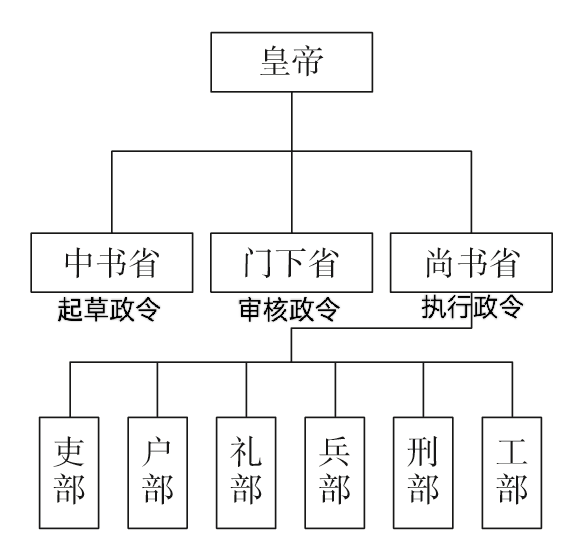
\includegraphics[scale=0.8]{img/201.png}
							\caption{三省六部制示意图}
						\end{figure} 
					\end{enumerate}
				\item 女皇帝武则天
					\begin{enumerate}
						\item 地位：中国历史上唯一的女皇帝。晚年称帝，改国号为周。
						\item 措施：
							\begin{enumerate}
								\item 打击\underline{\textbf{敌对的官僚贵族}}；
								\item 大力发展\underline{\textbf{科举制}}，创立\underline{\textbf{殿试制度}}；
								\item 继续推行贞观以来\underline{\textbf{减轻人民负担的政策}}，重视\underline{\textbf{发展生产}}。
							\end{enumerate}
						\item 治国成效：\underline{\textbf{为“开元盛世”局面的出现奠定了基础}}，后人称她的统治为“政起开元，治宏贞观”
					\end{enumerate}
				\item 唐玄宗与“开元盛世”（鼎盛时期）
					\begin{enumerate}
						\item 唐玄宗：李隆基，又称唐明皇，前期年号：开元。
						\item 措施；
							\begin{enumerate}
								\item 用人上：\underline{\textbf{重用贤能}}，任用贤相姚崇和宋璟。
								\item 政治上：整顿\underline{\textbf{吏治}}，裁减\underline{\textbf{冗员}}；
								\item 经济上：发展\underline{\textbf{经济}}，改革\underline{\textbf{税制}}；
								\item 文化上：注重\underline{\textbf{文教}}，编修\underline{\textbf{经籍}}。
							\end{enumerate}
						\item 治国成效：唐玄宗时期，唐朝进入\underline{\textbf{鼎盛时期}}，史称\underline{\textbf{“开元盛世”}}。
					\end{enumerate}
				\item 拓展：唐朝盛世局面两度出现给我们的启示：
					\begin{enumerate}
						\item \underline{\textbf{国家统一}}和\underline{\textbf{社会稳定}}是经济发展的前提条件；
						\item 治理国家要注重\underline{\textbf{人才的培养}}和\underline{\textbf{制度创新}}；
						\item 要重视发展经济，更要以民为本。
					\end{enumerate}
		\end{enumerate}
\end{document}